\documentclass{article}

\usepackage[utf8]{inputenc}
\usepackage[T1]{fontenc}      
\usepackage[francais]{babel}
\usepackage{graphicx}
\usepackage{circuitikz}
\usepackage[squaren, Gray]{SIunits}
\usepackage{sistyle}
\usepackage[autolanguage]{numprint}
\usepackage{pgfplots}
\pgfplotsset{compat=1.9}
\usepackage{amsmath,amssymb,array}
\usepackage[top=2.5cm,bottom=2.5cm,right=2.5cm,left=2.5cm]{geometry}
\usepackage{url} 
\usepackage{tabularx}
\DeclareMathOperator{\dist}{d}
\newenvironment{abstract-fr}
{
	\begin{center}
		\textbf{Résumé} \\[0.5cm]
	\end{center}
}
{}

\newenvironment{abstract-en}
{
	\begin{center}
		\textbf{Summary} \\[0.5cm]
	\end{center}
}
{}
% New command pour la modélisation mécanique, tri à effectuer
\newcommand\fv[1]{{\bf #1}} % free vector
\newcommand\fvd[1]{\dot{\bf #1}} % free vector derivated
\newcommand\fvdd[1]{\ddot{\bf #1}} % free vector derivated
\newcommand\fvr[1]{\mathring{\bf #1}} % free vector relatively derivated
\newcommand\fvrr[1]{\overset{\circ\circ}{\bf #1}} % free vector relatively derivated
\newcommand\uv[1]{{\bf\hat{ #1}}} % unit vector
\newcommand\ui{{\bf\hat{I}}} % unit vector I
\newcommand\uj{{\bf\hat{J}}} % unit vector J
\newcommand\uk{{\bf\hat{K}}} % unit vector K
\newcommand\wrt[2]{\ensuremath{\tensor*[_{ #1}]{ #2}{}}} % With Respect To
\newcommand\wtr[3]{\ensuremath{\tensor*[_{ #1}]{ #2}{^{ #3}}}} % With Two Respect
\newcommand\omegaf{{\bm \omega}}
\newcommand\omegafr{\mathring{\bm \omega}}
\newcommand\omegafd{\dot{\bm \omega}}
\newcommand\omegaft{\tilde{\bm \omega}}
\newcommand\omegaftr{\mathring{\tilde{\bm \omega}}}
\newcommand\omegat{\tilde{\omega}}
\newcommand\omegatd{\tilde{\dot{\omega}}}
\newcommand\ine{{\bf I}}
\newcommand\st{{\bf L}}
\newcommand\pst{{\bf M}}
\newcommand\lm{{\bf N}}
\newcommand\am{{\bf H}}
\newcommand\amd{\dot{\am}}
\newcommand\fo{{\bf F}}
\newcommand\po{\mathcal{P}}
\newcommand\xg{\ensuremath{\fv{R}}}
\newcommand\xgd{\ensuremath{\fvd{R}}}
\newcommand\xgdd{\ensuremath{\fvdd{R}}}
\newcommand\dvec[1]{\dot{\vec{ #1}}}
\newcommand\ddvec[1]{\ddot{\vec{ #1}}}
\newcommand\qp{\dot{q}}
\newcommand\dqp{\Delta \dot{q}}
\usepackage{url} 
\usepackage{hyperref}
\hypersetup{
    colorlinks,
    citecolor=black,
    filecolor=black,
    linkcolor=black,
    urlcolor=black
}

\begin{document}

\textbf{Groupe \numprint{11.53}}.

\section{Annexe documentaire}

\subsection{La contre-réaction ou réaction négative}

\paragraph{Choix du thème}
En analysant le circuit qui compose notre haut-parleur, nous avons remarqué
la présence de boucle reliant la sortie des amplificteurs à leur bornes négatives.
Nous nous sommes alors pourquoi ces boucles étaient là, et quels étaient leurs rôles
dans le cadre de notre haut-parleur. Après quelques recherches sur internet, nous avons
pu identifier ces boucles comme étant des boucles de contre-réaction ; nous avons
alors pu commencer notre recherche.

\paragraph{Mots clés et méthode de recherche}
Comme suggeré lors de la séance d'information sur la recherche bibliographique,
nous avons appliqué la méthode de l'entonnoir. Comme les boucles de contre-réaction 
sont directement liées aux amplificateurs, nous avons commencé nos recherches avec 
les termes plutôt généraux : \textit{amplificateurs} et \textit{amplifiers}. Nous 
nous avons ensuite associé à ces mots clés les termes plus précis : \textit{contre-réaction}
et \textit{negative feedback}.

Les différents ouvrages et documents que nous avons utilisés sont listés dans la bibliographie.

\paragraph{Quelques traces de notre recherche}
Voici quelques traces de notre recherches (Figures \ref{lynch1} et \ref{lynch2}), issues du livre 
\textit{Principle of electronic instrumentations},
par \textsc{Lynch} et \textsc{Truxal} aux éditions \textsc{McGraw-Hill}.

\begin{figure}[!htb]
	\centering
	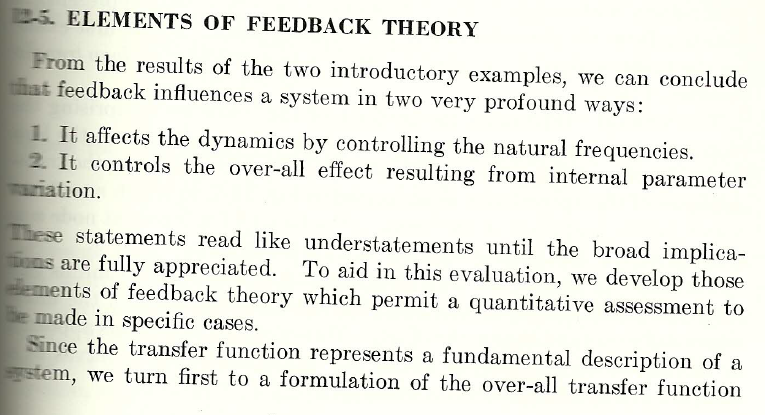
\includegraphics[scale=0.8]{lynch1.png}
	\caption{Page 670}
	\label{lynch1}
\end{figure}

\begin{figure}[!htb]
	\centering
	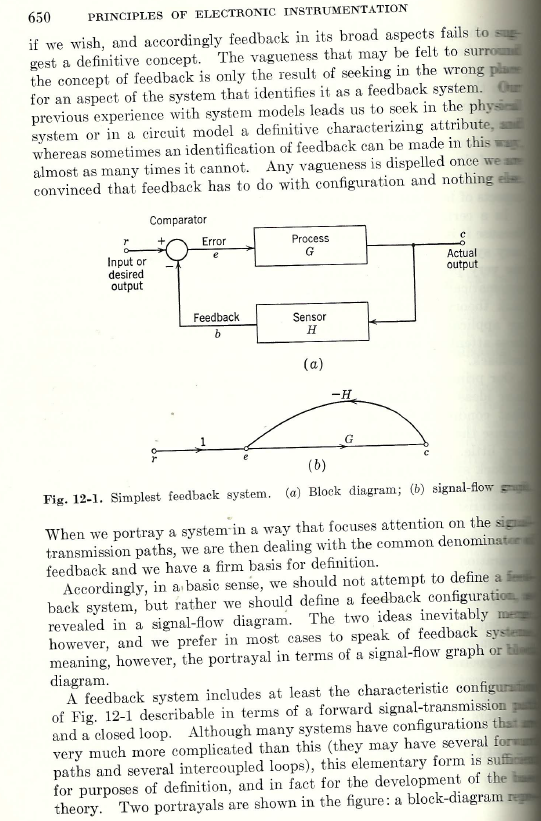
\includegraphics[scale=0.8]{lynch2.png}
	\caption{Page 650}
	\label{lynch2}
\end{figure}

\subsection{La distorsion harmonique}

\paragraph{Choix du thème}
Le choix du thème n'a pas été chose aisée. Nous avons commencé par établir un brainstorming afin de réunir 
le plus d'idées possibles. Cependant, les thèmes proposés nous semblaient trop généraux que pour faire un vrai 
travail en profondeur tout en restant concis. Quelqu'un a finalement proposé la distorsion harmonique ; un 
terme visible sur les emballages de haut-parleurs. Nous avions également repéré ce terme dans la datasheet 
de l'amplificateur audio reçu pour le projet: une valeur de \numprint{0.2}\% était renseignée pour le THD 
(taux de distorsion harmonique). Curieux d'en apprendre plus sur ce terme presque méconnu, 
nous avons décidé de débuter notre travail de recherche là-dessus.

\paragraph{Mots clés et méthode de recherche}
Etant donné que nous ne connaissions vraiment que très peu sur ce sujet et que nous 
devions le comprendre en profondeur, nous avons commencé par le terme général de "distorsion".
Une première recherche sur internet a permis de fixer les idées à propos de ce terme, et nous 
avons ensuite pu établir une liste de mot-clefs pour entamer réellement la recherche sur la 
distorsion harmonique. Nous avons appliqué la "technique de l'entonnoir", et nous avons finalement 
réuni assez d'informations que pour écrire ce rapport. Notons tout de même que c'est indiscutablement
en anglais que nous avons 
trouvé le plus d'informations. Nous avons gardé une trace de toutes les sources que nous avons 
consultées, et cela a rendu l'écriture de la bibliographie nettement plus facile.

\paragraph{Quelques traces de notre recherches}

\begin{figure}[!htb]
	\centering
	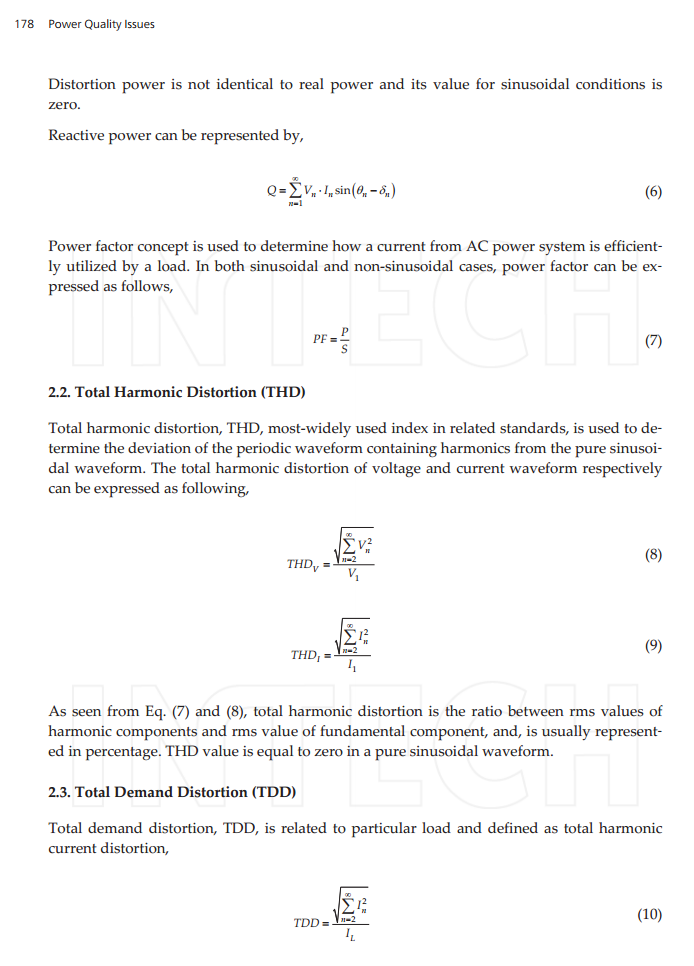
\includegraphics[scale=0.8]{thd.png}
	\caption{Celal Kocatepe, Recep Yumurtacı, Oktay Arıkan, Mustafa Baysal, Bedri Kekezoğlu, Altuğ Bozkurt and C. Fadıl KumruHarmonic,
					\textit{Effects Of Power System Loads : An experimental Study}, edition Intech.}
\end{figure}

\begin{figure}[!htb]
	\centering
	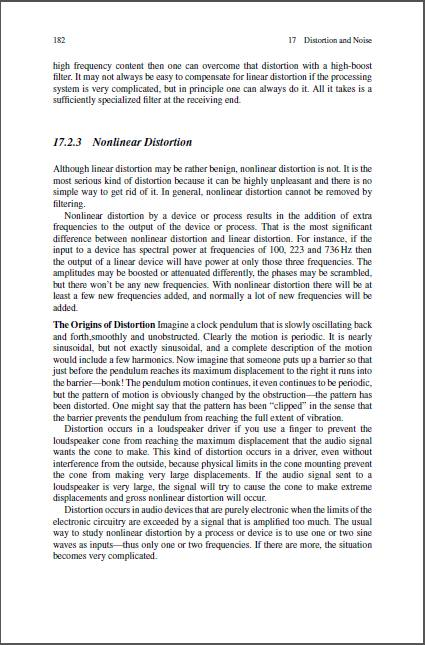
\includegraphics[scale=0.8]{distorsion1.jpg}
	\caption{Principles of musical acoustics, William M., Hartmann., Undergraduate Lecture Notes, Springer, New York.}
\end{figure}

\begin{figure}[!htb]
	\centering
	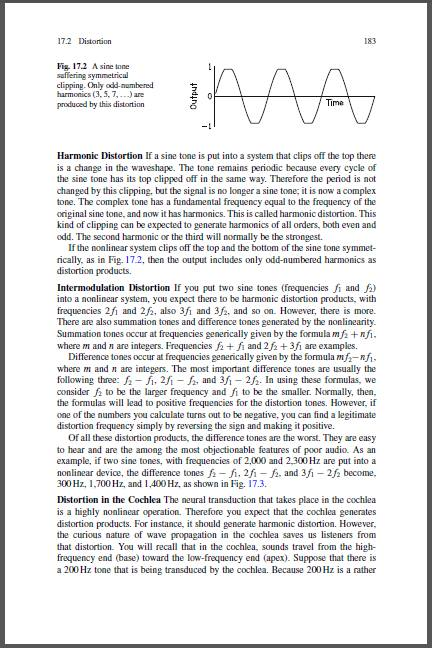
\includegraphics[scale=0.8]{distorsion2.jpg}
	\caption{Principles of musical acoustics, William M., Hartmann., Undergraduate Lecture Notes, Springer, New York.}
\end{figure}

% Just here to fix rapport_prejury.tex
\end{document}